\documentclass[xetex, unicode, 10pt]{beamer}
\usepackage{sty/style} 
\usepackage{lipsum}
\usepackage{amssymb}
\usepackage{amsmath}
\usepackage{pifont}% http://ctan.org/pkg/pifont
\newcommand{\cmark}{\ding{51}}%
\newcommand{\xmark}{\ding{55}}%
\newcommand\blfootnote[1]{%
  \begingroup
  \renewcommand\thefootnote{}\footnote{#1}%
  \addtocounter{footnote}{-1}%
  \endgroup
}


\title{
  Chisel Implementation Tutorial
}
\subtitle{In a lightweight and simple way}
\author{Rongwei\ Lin}
\institute{
  JLSemi Inc.
}
\date{\today}
\titlegraphic{
\includegraphics[width = 2cm]{fig/logo}} 

\begin{document}

\maketitle

\section{Data Type}

\begin{frame}
  \frametitle{Chisel Type}

  Chisel Type is abstract data type for Verilog.

  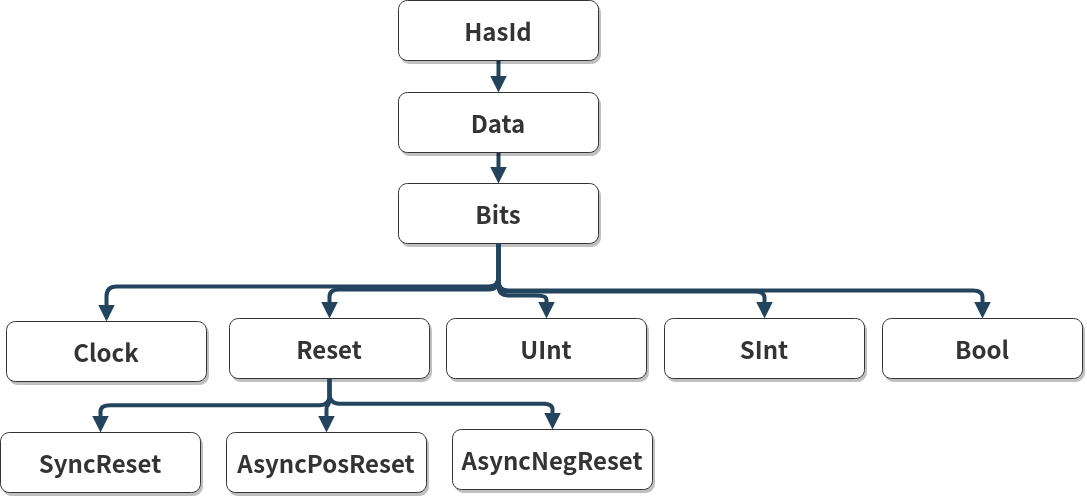
\includegraphics[width = 12cm]{./fig/datatype.png}
\end{frame}

\begin{frame}
  \frametitle{Hardware Type}

  Bind \Emph{Chisel Type} to \emph{Synthesizable} Verilog Type:

  \begin{block}{Constrained Binding}
    Used for connection, care about which module scope.
    \begin{itemize}
      \item OpBinding (read only)
      \item PortBinding
      \item RegBinding
      \item WireBinding
    \end{itemize}
  \end{block}

  \begin{block}{Unconstrained Binding}
    Not for connection, don't care about which module scope.
    \begin{itemize}
    \item LitBinding
    \end{itemize}
  \end{block}

\end{frame}

\begin{frame}
  \frametitle{Bits}

  \begin{itemize}
    \item Suggest Name: User specified
    \item Reference: associate with IR
    \item Binding: is Synthesizable
    \item Type: IR Type
    \item Direction: Input/Output/InOut
    \item Op Methods: +/-/\&/~ ...
  \end{itemize}

\end{frame}

\section{Statements}

\begin{frame}
  \frametitle{Statements}

  \Emph{Statements} create a kind of \emph{verilog} statement, such as:
    \begin{itemize}
      \item {Wire Declaration}
      \item {Register Declaration}
      \item {Connection}
    \end{itemize}

\end{frame}

\begin{frame}[fragile]
  \frametitle{Wire Declaration}
  Wires as hardware nodes to which one can assign values or connect other nodes.	

  \begin{block}{Wire()}
    \begin{columns}[T]
      \begin{column}{0.5\textwidth}
        \lstinputlisting [language = scala]{./code/wire.scala }
      \end{column}
      \begin{column}{0.5\textwidth}
        \lstinputlisting [language = verilog]{./code/wire.v }
      \end{column}
    \end{columns}
  \end{block}

  \begin{block}{WireInit()}
    \begin{columns}[T]
      \begin{column}{0.5\textwidth}
        \lstinputlisting [language = scala]{./code/wireinit.scala }
      \end{column}
      \begin{column}{0.5\textwidth}
        \lstinputlisting [language = verilog]{./code/wireinit.v }
      \end{column}
    \end{columns}
  \end{block}
\end{frame}

\begin{frame}
  \frametitle{Register Declaration}

  \begin{columns}[T]
    \begin{column}{0.5\textwidth}
      \Emph{Reg()}: without Reset
      \lstinputlisting [language = scala]{./code/reg.scala }
      \lstinputlisting [language = verilog]{./code/reg.v }
    \end{column}
    \begin{column}{0.5\textwidth}
      \Emph{RegInit()}: with \emph{Sync} Reset
      \lstinputlisting [language = scala]{./code/RegInitSync.scala }
      \lstinputlisting [language = verilog]{./code/RegInitSync.v }
    \end{column}
  \end{columns}

\end{frame}

\begin{frame}
  \frametitle{Register Declaration}

  \Emph{RegInit()}: with \emph{AsyncNeg} Reset
  \lstinputlisting [language = scala]{./code/RegInitAsyncNeg.scala }
  \lstinputlisting [language = verilog]{./code/RegInitAsyncNeg.v }

\end{frame}

\begin{frame}
  \frametitle{Register Declaration}

  \Emph{RegInit()}: with \emph{AsyncPos} Reset
  \lstinputlisting [language = scala]{./code/RegInitAsyncPos.scala }
  \lstinputlisting [language = verilog]{./code/RegInitAsyncPos.v }

\end{frame}

\begin{frame}
  \frametitle{Connection}

  \begin{enumerate}
    \item Context is same module of both sink and source
    \item Context is same module as sink and source is child module
    \item Context is same module as source and sink is child module
    \item Context is the parent module of both sink and source
  \end{enumerate}

  \begin{table}[h!]
  \footnotesize
  \centering
  \begin{tabular}{||c c c||}
    \hline
      Case & Sink & Source \\
    \hline\hline
      1 & Current MOD & Current MOD \\
      2 & Current MOD & Child   MOD \\
      3 & Child   MOD & Current MOD \\
      4 & Child   MOD & Child   MOD \\
    \hline
  \end{tabular}
  \caption{Four cases when connect source to sink.}
  \label{table:1}
  \end{table}

\end{frame}

\begin{frame}
  \frametitle{Connection: Case 1 \& 2}

  \Emph{case 1:} Context is same module of both sink and source

  \begin{table}[h!]
  \footnotesize
  \centering
  \begin{tabular}{||c c c||}
    \hline
      Case & Sink & Source \\
    \hline\hline
     \checkmark & Output   & \_\_\_ \\
     \checkmark & Internal & \_\_\_ \\
     \xmark     & Input    & \_\_\_ \\
    \hline
  \end{tabular}
  \end{table}

 \Emph{case 2:} Context is same module as sink and source is child module

  \begin{table}[h!]
  \footnotesize
  \centering
  \begin{tabular}{||c c c||}
    \hline
      Case & Sink & Source \\
    \hline\hline
     \checkmark & Internal & Output  \\
     \checkmark & Internal & Input   \\
     \checkmark & Output   & Output  \\
     \checkmark & Output   & Input   \\
     \xmark     & Input    & \_\_\_  \\
    \hline
  \end{tabular}
  \end{table}


\end{frame}

\begin{frame}
  \frametitle{Connection: Case 3 \& 4}

  \Emph{case 3:} Context is same module as source and sink is child module

  \begin{table}[h!]
  \footnotesize
  \centering
  \begin{tabular}{||c c c||}
    \hline
      Case & Sink & Source \\
    \hline\hline
     \checkmark & Input    & \_\_\_ \\
     \xmark     & Output   & \_\_\_ \\
     \xmark     & Internal & \_\_\_ \\
    \hline
  \end{tabular}
  \end{table}

 \Emph{case 4:} Context is the parent module of both sink and source

  \begin{table}[h!]
  \footnotesize
  \centering
  \begin{tabular}{||c c c||}
    \hline
      Case & Sink & Source \\
    \hline\hline
     \checkmark & Input    & Input  \\
     \checkmark & Input    & Output \\
     \xmark     & Output   & \_\_\_ \\
     \xmark     & Internal & \_\_\_ \\
    \hline
  \end{tabular}
  \end{table}

\end{frame}

\section{Module}

\begin{frame}
  \frametitle{Module}

  \Emph{Collect Ports} \\
  Through \raise1pt\hbox{\fbox{\lstinline[language=scala]|IO(...)|}} method. E.g: \raise1pt\hbox{\fbox{\lstinline[language=scala]|IO(Input(Bool())|}}

  \Emph{Collect Statements} \\
  Through statements API, such as  \raise1pt\hbox{\fbox{\lstinline[language=scala]|WireInit(10.U)|}}

  \Emph{Generate Component}
  \begin{enumerate}
    \item Get Name of \Emph{Bits} by \hbox{\fbox{\lstinline[language=scala]|[java.lang.reflect.Method]|}}
    \item Naming \Emph{Ports}
    \item Naming \EMPH{Synthesizable} \Emph{Bits}
    \item Generate \Emph{Circuit IR}
      \begin{itemize}
        \item Name
        \item Ports IR
        \item Statements IR
      \end{itemize}
  \end{enumerate}
\end{frame}

\section{IR}

\begin{frame}
  \frametitle{Circuit \& Component \& DefModule}

  \begin{columns}
    \begin{column}{0.5\textwidth}
      \begin{block}{Circuit}
        \begin{itemize}
	  \item name    \(\rightarrow\) \Emph{String}
	  \item modules \(\rightarrow\) \Emph{Component}
        \end{itemize}
      \end{block}
    \end{column}
    \begin{column}{0.5\textwidth}
      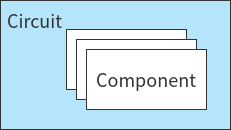
\includegraphics[width=3cm]{./fig/ir/circuit.png}
    \end{column}
  \end{columns}
  \begin{columns}
    \begin{column}{0.5\textwidth}
      \begin{block}{Component}
        \begin{itemize}
          \item name  \(\rightarrow\)  \Emph{String}
          \item ports \(\rightarrow\) \Emph{Port}
        \end{itemize}
      \end{block}
    \end{column}
    \begin{column}{0.5\textwidth}
      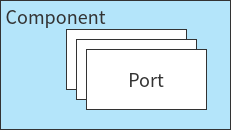
\includegraphics[width=3cm]{./fig/ir/component.png}
    \end{column}
  \end{columns}
  \begin{columns}
    \begin{column}{0.5\textwidth}
      \begin{block}{DefModule}
        \begin{itemize}
          \item name  \(\rightarrow\) \Emph{String}
          \item ports \(\rightarrow\) \Emph{Port}
	  \item stmts \(\rightarrow\) \Emph{Statement}
        \end{itemize}
      \end{block}
    \end{column}
    \begin{column}{0.5\textwidth}
      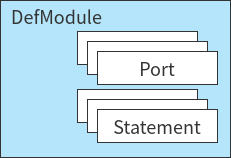
\includegraphics[width=3cm]{./fig/ir/defmodule.png}
    \end{column}
  \end{columns}

\end{frame}

\begin{frame}
  \frametitle{Port \& Direction}

  \begin{block}{Port}
    \begin{itemize}
      \item data      \(\rightarrow\) \Emph{Bits}
      \item direction \(\rightarrow\) \Emph{Direction}
    \end{itemize}
  \end{block}

  \begin{block}{Direction}
    \begin{itemize}
      \item {Input}
      \item {Output}
      \item {InOut}
    \end{itemize}

  \end{block}

\end{frame}

\begin{frame}
  \frametitle{Statement}

  \begin{block}{Statement}
    \begin{columns}
      \begin{column}{0.5\textwidth}
        \begin{itemize}
          \item {DefWire}
            \begin{itemize}
              \item e \(\rightarrow\) \Emph{Expression}
            \end{itemize}
          \item{Connnect}
            \begin{itemize}
              \item loc \(\rightarrow\) \Emph{Expression}
              \item expr \(\rightarrow\) \Emph{Expression}
            \end{itemize}
          \item{DefRegister}
            \begin{itemize}
              \item clock \(\rightarrow\) \Emph{Expression}
              \item reset \(\rightarrow\) \Emph{Expression}
              \item init  \(\rightarrow\) \Emph{Expression}
            \end{itemize}
        \end{itemize}
      \end{column}
      \begin{column}{0.5\textwidth}
      \end{column}
    \end{columns}

  \end{block}

\end{frame}

\begin{frame}
  \frametitle{Expression}

  \begin{block}{Expression}
    \begin{itemize}
      \item Reference
      \item Node
      \item DoPrim
      \item ILit
      \item Literal
        \begin{itemize}
          \item UIntLiteral
          \item SIntLiteral
        \end{itemize}
    \end{itemize}
  \end{block}

\end{frame}

\begin{frame}
  \frametitle{Expression}

  \begin{columns}
    \begin{column}{0.5\textwidth}
      \begin{itemize}
        \item Reference
          \begin{itemize}
            \item serialize \(\rightarrow\) \Emph{String}
            \item tpe       \(\rightarrow\) \Emph{Type}
          \end{itemize}

        \item Node
          \begin{itemize}
            \item id \(\rightarrow\) \Emph{Data}
          \end{itemize}

        \item DoPrim
          \begin{itemize}
            \item op     \(\rightarrow\) \Emph{PrimOp}
            \item args   \(\rightarrow\) \Emph{Seq[Expression]}
            \item consts \(\rightarrow\) \Emph{Seq[BigInt]}
          \end{itemize}
      \end{itemize}

    \end{column}
    \begin{column}{0.5\textwidth}
      \begin{itemize}
        \item ILit
          \begin{itemize}
            \item id \(\rightarrow\) \Emph{Data}
          \end{itemize}

        \item Literal
          \begin{itemize}
            \item {UIntLiteral}
              \begin{itemize}
                \item valude \(\rightarrow\) \Emph{BigInt}
                \item width  \(\rightarrow\) \Emph{Width}
              \end{itemize}
            \item{SIntLiteral}
              \begin{itemize}
                \item valude \(\rightarrow\) \Emph{BigInt}
                \item width  \(\rightarrow\) \Emph{Width}
              \end{itemize}
          \end{itemize}
      \end{itemize}
    \end{column}
  \end{columns}

\end{frame}

\begin{frame}
  \frametitle{Type}

  \begin{columns}[t]
    \begin{column}{0.5\textwidth}
      \begin{block}{Type}
        \begin{itemize}
          \item UIntType
            \begin{itemize}
              \item width \(\rightarrow\) \Emph{IntWidth}
            \end{itemize}
          \item SIntType
            \begin{itemize}
              \item width \(\rightarrow\) \Emph{IntWidth}
            \end{itemize}
          \item ClockType
            \begin{itemize}
              \item width \(\rightarrow\) \Emph{IntWidth(1)}
            \end{itemize}
          \item ResetType
            \begin{itemize}
              \item width \(\rightarrow\) \Emph{IntWidth(1)}
            \end{itemize}
            \begin{itemize}
              \item SyncResetType
              \item AsyncNegResetType
              \item AsyncPosResetType
            \end{itemize}
        \end{itemize}
      \end{block}
    \end{column}
    \begin{column}{0.5\textwidth}
      \begin{block}{Width}
        \begin{itemize}
          \item IntWidth
            \begin{itemize}
              \item value \(\rightarrow\) \Emph{BigInt}
            \end{itemize}
          \item UnknownWidth
            \begin{itemize}
              \item valude \(\rightarrow\) \Emph{BigInt}
            \end{itemize}
        \end{itemize}
      \end{block}
    \end{column}

  \end{columns}
\end{frame}



\section{Generate Verilog}

\begin{frame}
  \frametitle{Example}

  \lstinputlisting [language = scala]{./code/Simple.scala }
\end{frame}

\begin{frame}
  \frametitle{Collect Ports}
    
  e.g: \hbox{\fbox{\lstinline[language=scala]|val clk = IO(Input(Clock()))|}}

  \begin{enumerate}
    \item Clock() \rightarrow \EMPH{Bits}
      \begin{itemize}
        \item \Emph{Synthesizable:} Chisel Type
        \item \Emph{Type:} ClockType
        \item \Emph{Direction}: Internal
      \end{itemize}
    \item Input() \rightarrow \EMPH{Bits}
      \begin{itemize}
        \item \Emph{Synthesizable:} Chisel Type
        \item \Emph{Type:} ClockType
        \item \Emph{Direction}: Input
      \end{itemize}
    \item IO() \rightarrow \EMPH{Bits} \rightarrow \EMPH{Ports List}
      \begin{itemize}
        \item \Emph{Synthesizable:} Port Binding
        \item \Emph{Type:} ClockType
        \item \Emph{Direction}: Input
        \item \Emph{ref}: None
      \end{itemize}

  \end{enumerate}
\end{frame}

\begin{frame}
  \frametitle{Collect Statements}

  e.g: \hbox{\fbox{\lstinline[language=scala]|val bowl = withClockAndReset(clk,rst) { RegInit(5.U ) }|}}

  \begin{enumerate}
    \item withClockAndReset(..)
      \begin{itemize}
        \item \Emph{Clock:} clk
        \item \Emph{Reset:} rst
      \end{itemize}
    \item 5.U \rightarrow \EMPH{Bits}
      \begin{itemize}
        \item \Emph{Synthesizable:} Chisel Type
        \item \Emph{Type:} UIntType
        \item \Emph{Direction}: Internal
        \item \Emph{ref}: UIntLiteral
      \end{itemize}
    \item RegInit() \rightarrow \EMPH{DefRegister} \rightarrow \EMPH{Statements List}
      \begin{itemize}
        \item \Emph{Synthesizable:} RegBinding
        \item \Emph{Type:} UIntType
        \item \Emph{Direction}: Internal
        \item \Emph{ref}: UIntLiteral
      \end{itemize}
    \end{enumerate}
\end{frame}

\begin{frame}
  \frametitle{Generate Component}

  \Emph{1.Get Bits name}
  \begin{enumerate}
    \item Get Public Fields of \hbox{\fbox{\lstinline[language=scala]|Class|}}
    \item Filter \hbox{\fbox{\lstinline[language=scala]|HasId|}}, store delcared name.
  \end{enumerate}

  \Emph{2. Naming Ports}
  \begin{enumerate}
  \item Set each port of  \rightarrow  \EMPH{Ports List}
    \begin{itemize}
      \item \Emph{ref}: Reference(name)
    \end{itemize}
  \end{enumerate}

  \Emph{4. Naming Synthesizable Bits}
  \begin{enumerate}
    \item Name \Emph{Bits} if it does not \hbox{\fbox{\lstinline[language=scala]|suggestName|}}
    \item Set \hbox{\fbox{\lstinline[language=scala]|Reference(name, type)|}} IR to \Emph{Bits}
  \end{enumerate}

\end{frame}

\begin{frame}
  \frametitle{Generate Component}

  \Emph{5. Generate Circuit IR}
  \begin{itemize}
    \item \Emph{name:} class name as default
    \item \Emph{ports:} Port(clk, Input), 
      \begin{itemize}
        \item Port(clk, Input), 
        \item ...
      \end{itemize}
    \item \Emph{Statements}:
      \begin{itemize}
        \item DefRegister(Node(bowl), clk, rst, 5.U), 
	\item DefWire(Node(fruit))
	\item Connect(Node(fruit), Node(Bits(DoPrim(Or, [(sel \& apple), (~sel \& cherry)]))))
	\item Connect(Node(bowl), Node(Bits(DoPrim(Add, [bowl, fruit]))))
	\item Connect(Node(juice), Node(bowl))
      \end{itemize}
  \end{itemize}

\end{frame}

\begin{frame}
  \frametitle{Generate Verilog}

  \lstinputlisting [language = verilog]{./code/Simple.v }
\end{frame}


\begin{frame}[allowframebreaks, noframenumbering]{Thank You}
  \printbibheading[heading = none]
  \printbibliography
  \begin{block}{Talk is cheap. Show me the code.}
    \begin{itemize}
     \thusitem https://github.com/colin4124/Chisel-Implementation-Tutorial
    \end{itemize}
  \end{block}
  \blfootnote{
  Thanks for sano-jin: https://github.com/sano-jin/express-beamer
  }

\end{frame}

\end{document}
